\part{Práctica 4}
\section{Actividad 4-1}
\label{p41}
\begin{center}
    \parbox{12cm}{\justify\textit{Escoja una de las bases de datos de clasificación para el trabajo de las dispuestas en Moodle (Breast Cancer, Dermatology, Fantasmas, Glass, Vehicle, Wine, Zoo). \\
    Se entiende que además de pasarla a formato .arff ya ha aplicado el preprocesamiento necesario en función del fichero ``\textbf{Pistas sobre los datasets con posible preprocesamiento a simple vista.pdf}'', en el caso de que sea una de las bases de datos que lo requiera.
    \begin{itemize}
        \item Cargue la base de datos y ejecute el algoritmo \textbf{C4.5} usando un 75\% para entrenar y un 25\% para generalizar, con los parámetros por defecto.
        \item Analice y muestre el árbol obtenido con los parámetros por defecto: nodo principal, número de nodos u hojas, variables presentes y omitidas. Comente también los resultados de las métricas obtenidas.
    \end{itemize}
    }}
\end{center}

Para la realización de esta actividad se va a utilizar la misma base de datos preprocesada de la práctica 3 (fantasmas). El objetivo es construir en Weka un árbol de decisión mediante el algoritmo C4.5, para lo cuál utilizaremos el clasificador llamado ``J48'' en Weka. Tal como indica el enunciado, se divide el conjunto en dos, seleccionando un 75\% (278 patrones) para la construcción del árbol (train) y el 25\%restante (93 patrones) para generalización (test). Weka realiza esta división manteniendo idénticas frecuencias de las clases en cada subconjunto.

El algoritmo construye el árbol mediante un proceso recursivo en el que, para establecer cada nodo se busca el atributo con mayor porcentaje de ganancia de información ($I(C,X_i)/H(X_i)$), generando una partición en dos del conjunto de datos. En caso de que el atributo sea continuo, el algoritmo es capaz de determinar el mejor umbral. Para cada división del conjunto se añade una arista desde el nodo generado y se repite el proceso con el subconjunto correspondiente. Cuando todos los patrones asociados aun determinado recorrido en profundidad tienen la misma clase, se añade un nodo hoja. El algoritmo C4.5 también permite realizar podas que o bien sustituyen un sub-árbol por un nodo hoja o bien por una parte éste (elevación de sub-árbol). Es interesante mencionar que con este algoritmo, a diferencia de C3, sí que podemos encontrar varias veces el mismo atributo al realizar un recorrido del árbol en profundidad, al menos en el caso de atributos continuos y con diferentes umbrales.

Tal como podemos observar en la figura \ref{fig:j48-arbol}, en este caso de estudio, el atributo de mayor ganancia es hair\_length, por tanto se establece como nodo raíz. El árbol generado cuenta con 53 nodos, 27 de los cuáles son nodos hoja. Cada nodo hoja indica la cantidad de patrones del conjunto de generalización que, siendo de la clase indicada, han alcanzado el nodo así como la cantidad de patrones de otras clases que lo han alcanzado, en caso de haber alguno.

De los resultados del clasificador (fig. \ref{fig:j48-resultados}) podemos comentar que se han clasificado correctamente 65 patrones (69,89\%) de un total de 93 del conjunto de generalización. El estadístico Kappa es $\kappa=0,5473$, comparable aunque peor que el obtenido en los ensayos con otros tipos de clasificadores para el mismo conjunto de datos. La clase que peor se reconoce es de nuevo Goblin, con un TP Rate de 0,618, más elevado que el obtenido en los clasificadores anteriores, aunque hay que observar que en este caso, el FP Rate también es más alto, lo que da el peor resultado en AUC para todos los clasificadores utilizados con este conjunto. Esta comparación no es del todo justa porque se ha utilizado una técnica distinta para la generalización. En la matriz de confusión podemos ver que sólo 21 de los 34 Goblins han sido correctamente clasificados.

\begin{landscape}
\begin{figure}[!h]
    \centering
    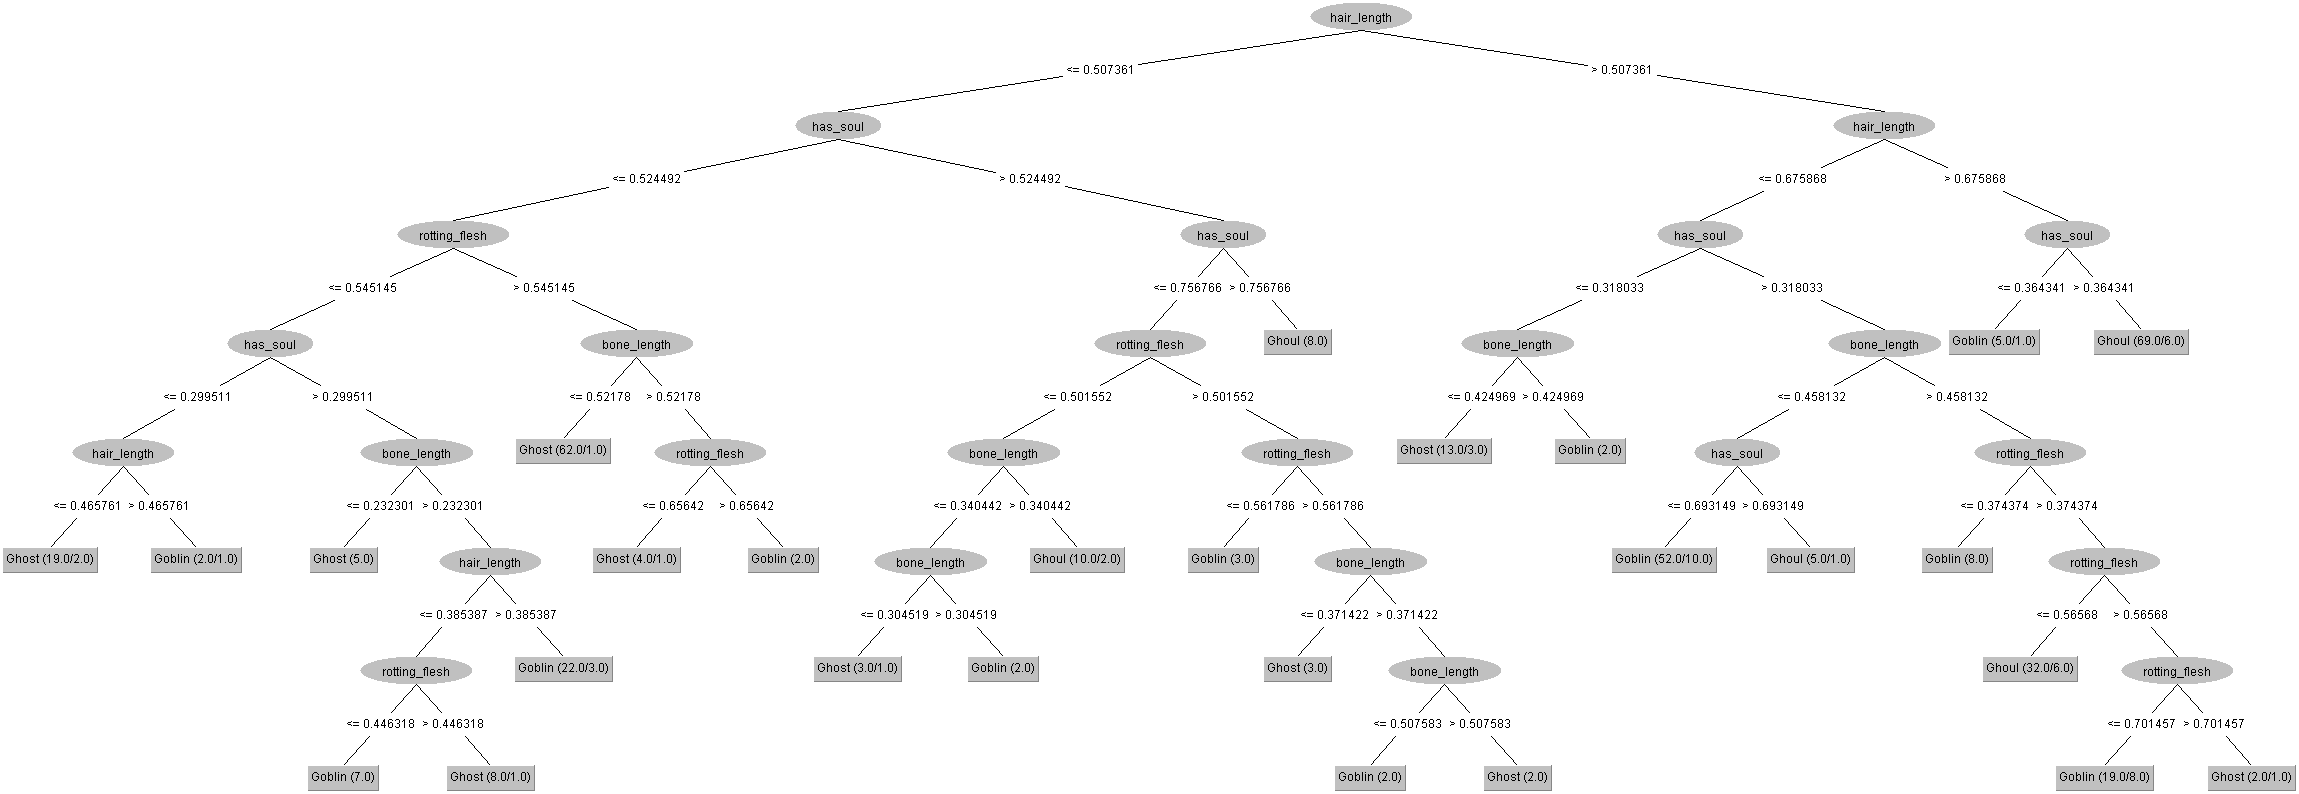
\includegraphics[height=0.5\textheight]{arbol}
    \caption{Árbol de decisión obtenido mediante C4.5}
    \label{fig:j48-arbol}
\end{figure}
\end{landscape}

\begin{figure}[ht]
    \centering
    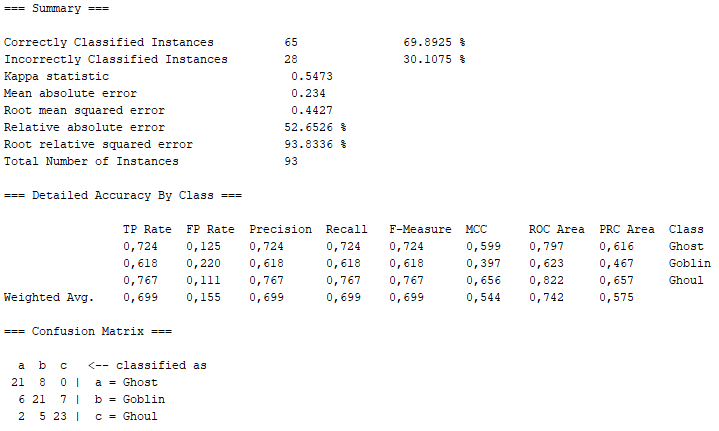
\includegraphics[width=\textwidth,keepaspectratio=true]{j48-resultados}
    \caption{Resultados del clasificador }
    \label{fig:j48-resultados}
\end{figure}


\clearpage
\section{Actividad 4-2}
\label{p42}
\begin{center}
    \parbox{12cm}{\justify\textit{Escoja una de las bases de datos de clasificación para el trabajo de las dispuestas en Moodle (Breast Cancer, Dermatology, Fantasmas, Glass, Vehicle, Wine, Zoo). \\
    Se entiende que además de pasarla a formato .arff ya ha aplicado el preprocesamiento necesario en función del fichero ``\textbf{Pistas sobre los datasets con posible preprocesamiento a simple vista.pdf}'', en el caso de que sea una de las bases de datos que lo requiera.
    \begin{itemize}
        \item Cargue la base de datos con un 75/25\% y ejecute el algoritmo Multilayer-Perceptron con los valores por defecto.
        \item ¿Qué observa al ir modificando sólo el \textbf{TrainingTime}? ¿Cambia el valor de Correctly Classified instances al modificar el parámetro? ¿Se estanca el aprendizaje o sobreentrena?
        \item ¿Qué observa al ir modificando sólo el \textbf{LearningRate}? ¿Cambia el valor de Correctly Classified instances al modificar el parámetro? ¿Se estanca el aprendizaje o sobreentrena?
    \end{itemize}
    }}
\end{center}